\chapter{Zoeken in zoekruimten}
\begin{itemize}
	\item Een zoekruimte tracht de manier van het menselijk redeneren na te bootsen.
	\item \underline{Drie elementen:}
	\begin{itemize}
		\item Een gerichte graaf, waarin de knopen toestanden zijn, en waarin er een verbinding van toestand $a$ naar toestand $b$ is als er in $a$ een actie mogelijk is die tot $b$ leidt.
		\item Een begintoestand.
		\item Een doel, dat bestaat uit een verzameling van toestanden.
	\end{itemize}
	\item Soms is het afgelegde pad belangrijk, bijvoorbeeld wanneer de kost ook belangrijk is.
\end{itemize}
\section{STRIPS}
\begin{itemize}
	\item \textbf{STanford Research Institute Problem Solver (STRIPS)} = een algemene probleemoplosser.
	\item Met behulp van een taal wordt het op te lossen probleem beschreven.
	\item \underline{Voorbeeld:} de torens van Hanoi (Figuur \ref{fig:torensVanHanoi}).
	\begin{figure}[h]
		\centering
		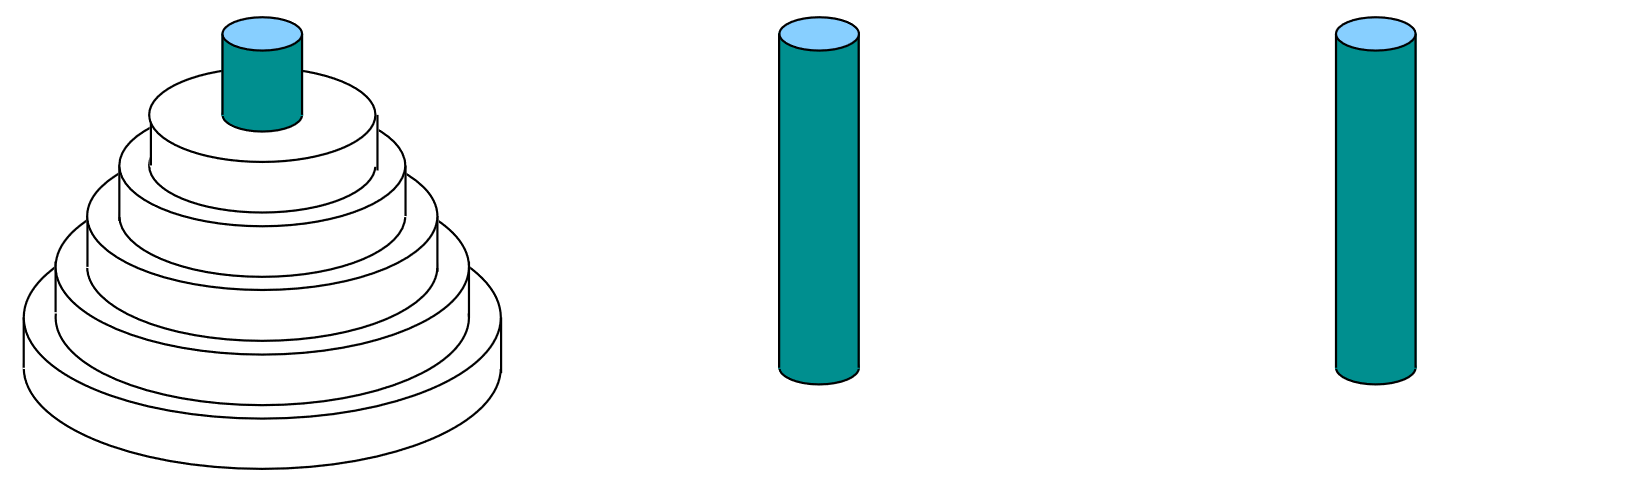
\includegraphics[width=\textwidth]{torensVanHanoi}
		\caption{De torens van Hanoi.}
		\label{fig:torensVanHanoi}
	\end{figure}
	\begin{itemize}
		\item Twee niveaus van positieve uitspraken:
		\begin{enumerate}
			\item Nuldeordepredicaten: Dit zijn strings, zoals \textit{DeLuchtIsBlauw} of \textit{Veilig}.
			\item Eersteordepredicaten: Deze zijn functies met een aantal parameters, die objecten aanduiden.
		\end{enumerate}
		\item Elke schijf hangt aan een bepaalde pin, er kan dus een predicaat van de eerste orde ingevoerd worden zoals bijvoorbeeld:
		$$\texttt{HangtAan(schijf1, pin1)}$$
		\item Ook moet duidelijk gemaakt worden dat twee verschillende pinnen effectief verschillend zijn:
		$$\texttt{IsNiet(pin1, pin2)}$$
		\item De begintoestand van de torens van Hanoi kan nu beschreven worden als volgt:
		\begin{equation*}
			\begin{split}
				\texttt{HangtAan(schijf1, pin1)}& \;\wedge \\
				\texttt{HangtAan(schijf2, pin1)}& \;\wedge \\
				\texttt{HangtAan(schijf3, pin1)}& \;\wedge \\
				\texttt{HangtAan(schijf4, pin1)}& \;\wedge \\
				\texttt{HangtAan(schijf5, pin1)}& \;\wedge \\
				\texttt{IsNiet(pin1, pin2)}& \;\wedge \\
				\texttt{IsNiet(pin1, pin3)}& \;\wedge \\
				\texttt{IsNiet(pin2, pin1)}& \;\wedge \\
				\texttt{IsNiet(pin2, pin3)}& \;\wedge \\
				\texttt{IsNiet(pin3, pin1)}& \;\wedge \\
				\texttt{IsNiet(pin3, pin2)}&  \\
			\end{split}
		\end{equation*}
		De predicaten worden gebonden met een logische EN. Ook is het nodig om de symmetrie te definiëren, aangezien STRIPS hier niets van af weet.
		\item Nu kan een actie gedefinieerd worden om een schijf te bewegen. Voor elke schijf moet dit apart gedaan worden. Hier wordt het uitgewerkt voor schijf 2:
		\begin{equation*}
			\begin{split}
				\texttt{Beweeg}&\texttt{Schijf2(van, naar, tussen)}: \\ 
				P : &\quad\texttt{IsNiet(van, naar)} \wedge \texttt{IsNiet(van, tussen)} \wedge \texttt{IsNiet(naar, tussen)}  \\
				    &\quad \texttt{HangtAan(schijf1, tussen)} \wedge \texttt{HangtAan(schijf2, van)} \\
				+ : &\quad \texttt{HangtAan(schijf2, naar)}\\
				- : &\quad \texttt{HangtAan(schijf2, van)}
			\end{split}
		\end{equation*}
		Elke actie bestaat uit een premisse $P$ die voldaan moet zijn vooraleer de actie kan uitgevoerd worden. De lijst van de toe te voegen uitspraken wordt aangeduid met het $+$ symbool en de lijst met de te verwijderen uitspraken worden aangeduid met het $-$ symbool.
		\item Om de symmetrie van de begintoestand op te lossen zou een actie \texttt{IsSymmetrie(A, B)} aangemaakt kunnen worden als volgt:
		\begin{equation*}
			\begin{split}
				\texttt{IsSym}&\texttt{metrie(A, B)}: \\ 
				P : &\quad \texttt{IsNiet(A, B)}\\
				+ : &\quad \texttt{IsNiet(B, A)}\\
				- : &\quad /
			\end{split}
		\end{equation*}
	\end{itemize}
\end{itemize}
\section{Efficiënt zoeken in zoekruimten}
\subsection{Breedte-eerst zoeken}
\begin{itemize}
	\item De \textbf{vertakkingsfactor} is het gemiddeld aantal nieuwe, nog niet bekeken buren van een onderzochte knoop en wordt voorgesteld door $b$ (branching factor).
	\item Bij de torens van Hanoi is $b \approx 1,5$.
	\item Voor een diepte $d$ worden ongeveer 
	$$1 + b + b^2 + ... + b^d = \frac{b^{d + 1} - 1}{b - 1}$$
	knopen bezocht. Voor $b$ voldoende groter dan $1$ is dit ongeveer $b^d$.
	\item Als we tien zetten voor elke speler willen vooruitkijken bij schaken, moeten er $6^{20} \approx 3.6\cdot10^{15} = 3,6$ biljard knopen ontwikkeld worden.
	\item Indien zowel start- als eindtoestand bekend zijn, kan \textbf{bidirectioneel zoeken} toegepast worden. Er wordt vooruit gezocht vanuit het startpunt, en achteruit vanuit het doel, beide met breedte-eerst zoeken. Er moet dan in plaats van $b^d$ knopen slechts $2b^{d/2}$ knopen ontwikkeld worden. Voor $b = 2$ en $d = 20$ krijgen we met breedte-eerst zoeken $10^6$ knopen en met bidirectioneel zoeken ongeveer 2000.
\end{itemize}
\subsection{Heuristieken}
In plaats van breedte-eerst zoeken te gebruiken zou ook een manier kunnen gebruikt worden die de meest interessante knoop volgt, in plaats van ze blindelings af te lopen.
\begin{itemize}
	\item Bij het zoeken in een graaf worden er aan elke knoop $k$ twee waarden toegekend:
	\begin{enumerate}
		\item De gekende kost $g(k)$ van de knoop: 
		\begin{itemize}
			\item Deze functie is een schatting van de werkelijke kost $g^*(k)$ van het kortste  pad van de startknoop naar $k$.
			\item Het wordt berekend door bij de kost van zijn voorganger $v$ de kost $c(v \rightarrow k)$ op te tellen; de kost van de actie die $v$ omzet in $k$.

			\item Er geldt steeds $g(k) \geq g^*(k)$.
		\end{itemize} 
		\item De heuristische kost $h(k)$ van de knoop:
		\begin{itemize}
			\item Deze functie is een schatting van $h^*(k)$, de kost om vanuit de knoop het doel te bereiken via het kortste pad.
		\end{itemize}
	\end{enumerate}
	\item De som van deze twee waarden geven de geschatte kost, verpakt door de evaluatiefunctie $f$:
	$$f(k) = g(k) + h(k)$$
	\alert Interessante knopen heben een lage $f$ waarde. 
	\item \textbf{Beste-eerst zoeken}:
	\begin{enumerate}
		\item[(1)] Steek de startknoop $s$ in de verzameling niet-ontwikkelde knopen NOK met $g(s) = 0$. Geef alle andere knopen een voorlopige schatting $g(k) = \infty$.
		\item[(2)] Als NOK leeg is stop dan zonder oplossing, ga anders naar (3).
		\item[(3)] Zoek de knoop $k$ uit NOK met de laagste evaluatiewaarde en verwijder hem uit NOK.
		\item[(4)] Als $k$ in het doel zit, geef het pad naar $k$ terug en stop; ga anders naar (5).
		\item[(5)] Voor elke buur $b$ van $k$: bereken $g_k(b) = g(k) + c(k \rightarrow b)$ en vergelijk $g_k(b)$ met de voorlopige waarde die $g(b)$ al gekregen had. Als $g_k(b) < g(b)$, vervang dan $g(b)$ door $g_k(b)$ en steek $b$ in NOK als $b$ daar niet in zit.
		\item[(6)] Ga terug naar (2).
	\end{enumerate}
	\item De functie $g$ is afhankelijk van het probleem, maar $h$ hoeft dit niet te zijn. Er zijn verschillende mogelijkheden voor $h$. Er is wel de voorwaarde dat ze \textbf{toelaatbaar} moeten zijn. Dit wil zeggen dat het een pad vindt en dat dit pad optimaal is.
\end{itemize}
\subsubsection{A* heuristieken}
\begin{itemize}
	\item Een heuristiek is $A*$ als $h(k) \leq h^*(k)$.
	\item \underline{Bewijs:} indien er slechts een eindig aantal knopen $k_i$, met $g^*(k_i) \leq g^*(D)$ zijn, is een $A*$-heuristiek toelaatbaar.
	\begin{itemize}
		\item Neem een $A*$ heuristiek $h$ en bewijs dat er steeds een knoop $k'$ is die voldoet aan de volgende voorwaarden:
		\begin{enumerate}
			\item[(1)] $k'$ zit in NOK.
			\item[(2)] $k'$ ligt op een optimaal pad van $s$ naar $D$.
			\item[(3)] De schatting $g(k')$ is correct: $g(k') = g^*(k')$.
		\end{enumerate}
	\item Dit is geldig indien $k'$ de startknoop is. Er is minstens één buur $k''$ die ook op het optimale pad ligt. Door $k'$ te ontwikkelen wordt zijn plaats ingenomen door zijn opvolger $k''$ op het optimale pad.  $k''$ voldoet aan (3), want
	$$g^*(k'') = g(k') + c(k' \rightarrow k'') = g_{k'}(k'')$$
	\item Als $k'$ de laatste knoop op het pad is die aan de voorwaarden voldoet dan is de nieuwe $g(k'')$-waarde kleiner dan de vorige en komt $k''$ zeker in NOK. Bovendien geldt
	
	$$f(k') = g(k') + h(k') \leq g^*(k') + h^*(k') = g^*(D)$$
	
	\item Er kan geen enkele $k$ ontwikkeld worden met $g(k) > g^*(D)$, want dan zou $f(k) > f(k')$ zijn.
	\item Iedere keer als een knoop $k$ ontwikkeld wordt, is er een kleinere waarde voor $g(k)$ die overeenkomt met de kost van een pad $s$ naar $k$.
	\item Ooit zal een doelknoop $d$ gekozen worden voor ontwikkeling en die heeft $g(d) = f(d) \leq g^*(D)$, en is bijgevolg optimaal.
	\end{itemize}
\end{itemize}

\subsubsection{Monotone heuristieken}
\begin{itemize}
	\item Een heuristiek is monotoon als 
	\begin{enumerate}
		\item voor elk paar knopen geldt dat $h(v) - h(k) \leq c(v \rightarrow k)$.
		\item $h(d) = 0$ voor alle $d$ in de doelverzameling $D$.
	\end{enumerate}
	\item \underline{Bewijs:} Neem een willekeurig pad $k_0k_1, ...,k_n$ tussen twee knopen $k_0$ en $k_n$. Dan is de functie $g(k_i) + h(k_i)$ monotoon stijgend als functie van $i$. Hierin wordt $g(k_i)$ gerekend langs het pad vanaf het startpunt $k_0$.
	\begin{itemize}
		\item Voor $i < n$ geldt dat $g(k_i) + c(k_i \rightarrow k_{i + 1}) = g(k_{i + 1})$
		\item Ook geldt er dat $h(k_i) \leq h(k_{i + 1}) + c(k_i \rightarrow k_{i + 1})$.
		\item Deze twee termen optellen en de term $c(k_i \rightarrow k_{i + 1})$ schrappen levert 
		$$g(k_i) + h(k_i) \leq g(k_{i + 1}) + h(k_{i + 1})$$
	\end{itemize}
	\item \underline{Twee gevolgen:}
	\begin{enumerate}
		\item Een monotone heuristiek is $A*$.
		\item Een knoop $k$ wordt nooit ontwikkeld voor $g^*(k)$ gekend is.
	\end{enumerate}
	\item Efficiëntie
	\begin{itemize}
		\item Voor $h = 0$ krijgen we breedte-eerst zoeken.
		\item Voor $h = h*$ krijgen we de optimale heuristiek, die rechtstreeks naar het doel leidt, en die ook monotoon is.
		\item Hoe bepalen of een willekeurige monotone heuristiek beter is dan een andere?
		\begin{itemize}
			\item Laatste ontwikkelde knoop is altijd $d$ met $g^*(d) = g^*(D)$ en $h(d) = 0$.
			\item Voor een monotone heuristiek moeten alle knopen ontwikkeld worden waarvoor $g^*(k) + h(k) < g^*(D)$, en geen enkele waarvoor $g^*(k) + h(k) > g^*(D)$.
			\item Een monotone heuristiek $h_1$ ontwikkelt minder knopen dan een monotone heuristiek $h_2$ als $h_1(k) > h_2(k)$. 
			\item Als voor sommige $k$ geldt dat $h_1(k) < h_2(k)$ en voor andere $k$ $h_1(k) > h_2(k)$, kan een betere heuristiek opgebouwd worden:
			
			$$h_3 = \max\{h_1(k), h_2(k)\}$$
		\end{itemize}
		
	\end{itemize}
\end{itemize}

\subsubsection{Relaxatieheuristieken}
\begin{itemize}
	\item Worden bekomen door het originele probleem sterk te vereenvoudigen.
	\item Er worden verbindingen toegevoegd in de graaf, wat overeenkomt met het schrappen van acties in de premisse.
	\item Het kortste pad in nieuwe graaf is zeker niet langer dan het kortste pad in de originele graaf. Deze heuristiek is dan ook $A^*$.
\end{itemize}

\section{Spelbomen}
\begin{itemize}
	\item Wat doen indien er geen volledige kennis is over het resultaat van acties?
	\item Een \textbf{nulsomspel} (Engels: two player zero sum game)
	\begin{itemize}
		\item Twee spelers.
		\item Enkel winst mogelijk ten koste van de andere speler.
		\item De winst van de ene speler is gelijk aan het verlies van de andere speler.
		\item Elke speler probeert zijn winst te maximaliseren.
	\end{itemize}
	\item \underline{Voorbeeld van een nulsomspel:}
	\begin{itemize}
		\item Op een tafel tussen twee spelers liggen een aantal stapels jetons.
		\item De speler die aan de zet is moet een stapel nemen, en deze verdelen in twee ongelijke stapels.
		\item De speler die niet meer kan zetten verliest.
		\item De winnaar krijgt als winst het aantal punten gelijk aan het aantal overblijvende stapels, en de verliezer verliest dan ditzelfde aantal punten.
		\item Er kan een bijhorende boom (figuur \ref{fig:spelboom}) opgesteld worden die alle mogelijke zetten beschrijft.
		\begin{figure}
			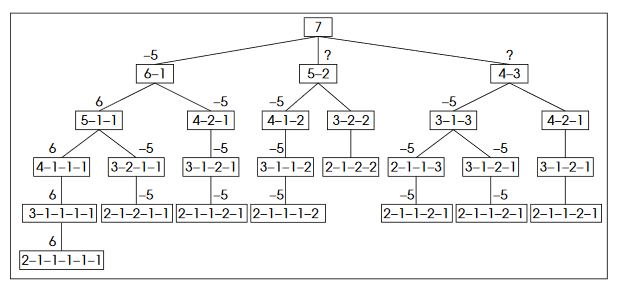
\includegraphics[width=\textwidth]{spelboom}
			\caption{Een spelboom waarbij de startsituatie een stapel van 7 jetons is.}
			\label{fig:spelboom}
		\end{figure}
		\item Noem de speler die begint \textit{Max}, en de andere speler \textit{Min}.
		\item Bij elke eindpositie is de winst of verlies van Max berekent.
		\item De overige posities kunnen van onder naar boven opgesteld worden:
		\begin{enumerate}
			\item Als Max aan zet is dan nemen we de grootste score.
			\item Als Min aan zet is nemen we de kleinste score.
		\end{enumerate} 
		\item Dit heet \textbf{minimax}. 
		\item Er wordt gebruik gemaakt van \textbf{$\alpha-\beta$ snoeien} om oninteressante zetten (deelbomen) zeker niet te evalueren in de spelboom. Op die manier is er minder geheugen nodig.
		\begin{itemize}
			\item De zet $7\rightarrow6-1$ levert een score van $-5$ op.
			\item Van de zet $7\rightarrow5-2$ weten we niet wat de score is.
			\begin{itemize}
				\item We weten wel dat Min erop kan reageren met een zet die een score van $-5$ geeft.
				\item Het kan zijn dat de andere deelboom een betere score oplevert voor Min, maar het zal zeker geen lagere zijn (want die zet zou hij niet nemen).
				\item Deze zet is niet beter dan $7\rightarrow 6 - 1$	
		\end{itemize}
			\item Algemeen wordt er gezocht naar een pad naar een blad waarbij zowel Max als Min steeds de beste zet kiezen.
			\begin{itemize}
				\item Op dit pad is de kost van alle knopen gelijk.
				\item De kost is $s_{opt}$, de optimale score.
			\end{itemize}
		\end{itemize}
		\item Moeten alle knopen ge-evalueerd worden om de optimale score te vinden?
		\begin{itemize}
			\item Een \textbf{voorbroer} $b$ van een knoop $k$ is een broer van $k$, of een broer van één van de voorouders van $k$ (Figuur \ref{fig:voorbroers}).
			\begin{figure}
				\centering
				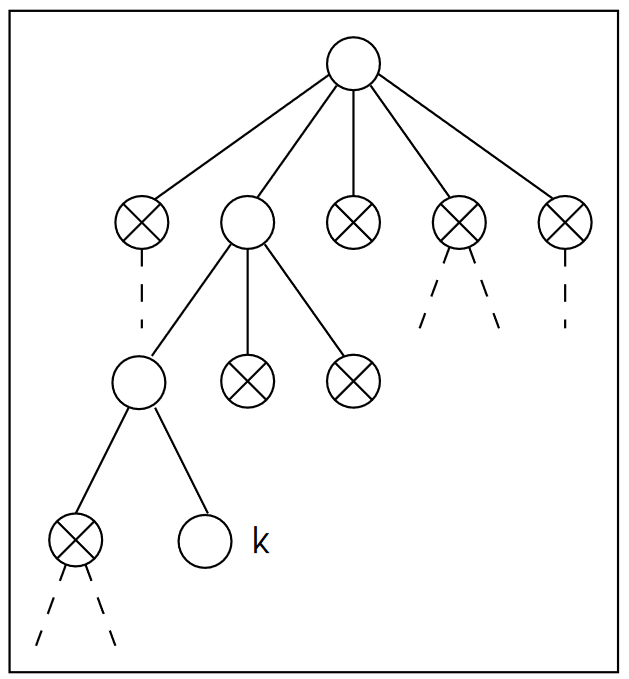
\includegraphics[width=0.5\textwidth]{voorbroers}
				\caption{De voorbroers van een knoop $k$ worden gemarkeerd met een kruis.}
				\label{fig:voorbroers}
			\end{figure}
			\item Neem een knoop $k$ en veronderstel dat $s(k)$ kan vervangen worden door een schatting $f$.
			\item De waarden van de voorouders van $k$ kunnen ook nu veranderd worden. Stel $f > s(k)$:
			\begin{enumerate}
				\item $k$ is een minknoop. Als $f >  s(b)\;\forall\;b \hbox{ broer van } k$, dan wordt de $s$-waarde van de ouderknoop vervangen door $f$. Nu wordt naar geval 2 gegaan.
				\item $k$ is een maxknoop en geen wortel. De nieuwe $s-$waarde van de ouder is hoogstens $f$. Nu wordt naar geval 1 gegaan.
			\end{enumerate}
		\end{itemize}
	\end{itemize}
\end{itemize}